\chapter{Implementation}
\label{cha:implementation}

This chapter describes how the concepts outlined previously were translated into practical solutions within the MS.
It details the key technical details involved in integrating environments,
folder structures,
user management,
and the enhancements made to the role-based access control system.
The implementation ensures robust isolation between environments and 
aims to achieve high maintainability and simplicity to support ongoing development.

% TODO: either finish this or remove it
% Additionally, the MS stores XML files for BPMN Assets.

\section{Users}

The user management in the MS was completely reworked to support the new 
environments design structure.
Users are now stored in a separate file in the MS' storage solution and are independent of
any environment.
Additionally, guest users were added to the MS to allow users to try the MS without
signing in with their personal information.

%
% \begin{lstlisting}[
%   language=JavaScript,
%   style=codestyle,
%   caption={Example setup of NextAuth.js.},
% ]
% const handler = NextAuth(nextAuthOptions);
% \end{lstlisting}

% TODO: this section
\subsection{Sign In Flows}

User authentication is implemented by leveraging OpenID Connect\ref{cha:relatedwork:oauth:openid},
with the help of the NextAuth.js\footnote{\url{https://next-auth.js.org/}} library.
A JWT token\footnote{\url{https://www.rfc-editor.org/rfc/rfc7519.txt}}
is stored in the user's browser cookies\footnote{\url{https://www.rfc-editor.org/rfc/rfc7519.html}},
which is then parsed and verified by the MS' backend.
This token contains the user's ID.
% TODO: is "id" the correct word here
If a user makes a request to the backend,
with a valid JWT token the user is considered authenticated.
If a user couldn't be authenticated, they're redirected to the sign-in page.

NextAuth.js has many sign-in methods built-in, which can be set up with little configuration.
For email-sign in, NextAuth.js sends an email with a link to the MS' backend with a token. 
When the backend receives this token, the user's cookies are set, and they're authenticated.
% We have to provide a way to store and query the tokens, that are encoded in the link and a
% function that sends the email.
% For OAuth2 providers, we only have to provide a client ID and secret.

%To store and look up users and accounts, NextAuth.js requires a database adapter,
%which is a set of functions that interact with the database.
%% TODO: add ref
%The structure of the data that will be stored described in \ref{}.

NextAuth.js provides hooks that allow us to customize the sign-in flow, the most important
one for this thesis is the \lstinline{signIn} hook.
This hook is called when a user tries to sign in, this can be a new user or a returning
one.
As arguments, the \lstinline{signIn} hook receives the user's data,
and the account that the user is trying to sign in with,
if the user doesn't exist the user data may be empty.
If the hook returns true, the sign-in flow continues, if it returns a string or false,
then the sign-in flow is stopped, and the user is redirected to an error page.
% Inside this hook, we can also check if the user was previously signed-in as a guest user
% and is now signing in with personal information, so that we can merge the data of the two,
% we will elaborate on this in \ref{cha:ms-architecture:merge-guest-user-data}.

% TODO: decicde if we need a setup example for nextauth.js
%\begin{lstlisting}[
%  language=JavaScript,
%  style=codestyle,
%  caption={Setup example for NextAuth.js.},
%]
%import NextAuth from 'next-auth/next';
%import GoogleProvider from 'next-auth/providers/google';
%
%const authOptions = {
%  providers: [
%    EmailProvider({
%      sendVerificationRequest({ url }) {
%        // send email
%      },
%    }),
%    GoogleProvider({
%      clientId: process.env.GOOGLE_CLIENT_ID,
%      clientSecret: process.env.GOOGLE_CLIENT_SECRET,
%    }),
%  ],
%}
%
%const handler = NextAuth(authOptions)
% \end{lstlisting}


% (property) signIn?: ((params: {
%     user: User | AdapterUser;
%     account: Account | null;
%     profile?: Profile | undefined;
%     email?: {
%         verificationRequest?: boolean | undefined;
%     } | undefined;
%     credentials?: Record<string, CredentialInput> | undefined;
% }) => Awaitable<string | boolean>) | undefined
%
% Use this callback to control if a user is allowed to sign in.
% Returning true will continue the sign-in flow.
% Throwing an error or returning a string will stop the flow, and redirect the user.
%
% [Documentation](https://next-auth.js.org/configuration/callbacks#sign-in-callback)


\subsection{Authenticated Users}
\label{cha:ms-architecture:authenticated-users}

Authenticated Users are users that sign in to the MS either with their email or with a
OAuth 2.0 provider.
They're stored in the MS after they have successfully signed in.
For authenticated users we store an ID, a flag named \lstinline{isGuest}, set
to false, and their personal information.
This is the schema for authenticated users:

% NOTE: maybe explain that because of nextauths weirdness the email is just stored in the
% user instead of the account

\begin{lstlisting}[
  language=JavaScript,
  style=codestyle,
  caption={Schema for authenticated users.},
  label={lst:authenticated-users-schema}
]
{
    id: string;
    isGuest: false;
    firstName?: string | undefined;
    lastName?: string | undefined;
    username?: string | undefined;
    image?: string |  undefined;
    email?: string | undefined;
}
\end{lstlisting}

All the personal information is optional, because depending on how the user signs in, the
information might not be available, when the user is created.
% For instance, because NextAuth.js' email sign in only requires the user to input an
% email, authenticated users are created without a first name, last name or username.
% A possible workaround would be to automatically generate these, but we chose to leave them
% undefined, and prompt the user to fill them when he first signs in.
After the user is created, if he has missing information, we prompt him to fill it in.

\begin{figure}[H]
	\centering
	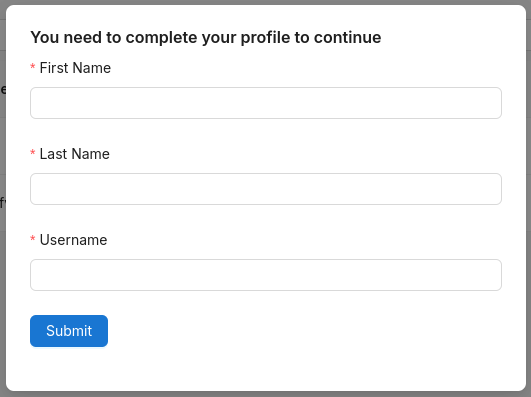
\includegraphics[scale=0.4]{images/fill-data-prompt.png}
	\caption{Prompt to fill in personal information.}
	\vspace{-1em} % Negative value to remove space
	\label{fig:prompt-fill-personal-information}
\end{figure}

% TODO: cite paper or something to show that this can happen?? im sure there's going to be
% smth
The \lstinline{image} field is used to store a URL to a user's profile picture. 
This field can only be set if the user signed in with an OAuth 2.0 provider,
that provided a profile picture URL.
We don't accept custom URLs,
as this allows for attackers to supply URLs to a server they control,
which can be used to track other user's browsers.
By only saving URLs provided by trusted OAuth 2.0 providers, we ensure that the
source of the image is reliable.

As stated before, Accounts are used to link sign-in data provided by OAuth 2.0 providers
after someone signs in, to a user in the MS.
Oauth 2.0 providers provide a unique ID for the user that signed in,
to recognize a user's account we need to store this ID and
the name of the provider.
Additionally, to link the account to a user, we store the user's ID in the MS.
The schema for accounts is as follows:

\begin{lstlisting}[
  language=JavaScript,
  style=codestyle,
  caption={Schema for accounts.},
  keywords={string}
]
{
    id: string;
    type: "oauth";
    userId: string;
    provider: string;
    providerAccountId: string;
}
\end{lstlisting}

\subsection{Guest Users}

Users that aren't signed in can choose to use the MS as a guest, this doesn't require
the user to input any personal information.
For these users, a new user is created and stored in the MS.
These users only store a unique ID and a flag named \lstinline{isGuest}, set to true.
% To achieve this, we use a modified version of the authenticated user schema described in
% \ref{lst:authenticated-users-schema}, to only include the \lstinline{id} and the
% \lstinline{isGuest} flag set to true.
% Additionally, guest users can store a reference to an authenticated user, named
% \lstinline{signedInWithUserId}, the purpose of this is explained in \ref{cha:ms-architecture:merge-guest-user-data}.

\begin{lstlisting}[
  language=JavaScript,
  style=codestyle,
  caption={Schema for guest users.},
]
{
    isGuest: true;
    id: string;
} 
\end{lstlisting}

% This option must be made available to users during the sign-in process.
% To accomplish this, NextAuth.js provides a built-in \lstinline{CredentialsProvider},
% which enables the implementation of custom sign-in methods.
% We configured this provider to accept no credentials,
% allowing users to sign in without supplying personal information.
%
% \begin{lstlisting}[
%   language=JavaScript,
%   style=codestyle,
%   caption={Custom sign-in method for guest users.},
% ]
% import NextAuth from 'next-auth/next';
%
% const authOptions = {
%   providers: [
%     ...
%     CredentialsProvider({
%       name: 'Continue as Guest',
%       credentials: {},
%       async authorize() {
%         return addUser({ isGuest: true });
%       },
%     }),
%   ],
% }
%
% const handler = NextAuth(authOptions)
% \end{lstlisting}

After a user signs in as a guest, a JWT token pointing to a real user is stored in his
cookies, so he can use the MS like an authenticated user.
Since there is no personal information stored, there is no way for the user to sign in to
his guest user from another device.
This also means, that if the JWT cookie is deleted, the user will lose access to his guest
user.

\subsection{Enforcement of limits for guest users}

Guests can have their own personal space for their assets, but they aren't allowed to create or join organization environments.
The system specifically prevents these actions in the corresponding endpoints, by checking
the \lstinline{isGuest} flag.
Consequently, any features inside an organization environment are inaccessible to guest users.


% TODO: subsection title :(
\subsection{Merging Guest User's Data with an Authenticated User's Data}
\label{cha:ms-architecture:merge-guest-user-data}

As explained in \ref{cha:conceptanddesign:users:guestuserstorage}, a guest user can sign in with an email or an OAuth 2.0 provider.
Once signed in, the \lstinline{isGuest} flag is set to false, and the user’s sign-in method is stored.
Since the user ID doesn't change, there’s no need to transfer existing assets.
If the chosen account is already linked to another user in the MS,
then the user is redirected to a page where he can choose to either transfer the guest user's assets to his 
already existing account or discard them.
This page takes a JWT token as a query parameter, which is generated after the user signs
in.
In the case of an Email sign-in, the token is generated by the MS when the user requests
the sign-in link, and added to the sign-in link as a URL that will be called after
authenticating the user.

we store a \lstinline{signedInWithUserId} value to reference that user.
This reference is needed, for the case that a user tries to sign in with an email, a
This flag is needed to prevent the attack shown in ????? where a user could hijack a guest
account's data through manipulating the
Afterward, the user can decide whether to transfer the guest’s assets to their personal environment or discard them.

Guest users can choose to sign in with their email or with an OAuth 2.0 provider.
By doing so, their guest user is turned into an authenticated user.
The \lstinline{isGuest} flag is set to false, and their sign-in method is stored.
All their assets don't need to be transferred, as they are already stored in the MS, and
the user ID wasn't changed.
This approach only works if the account that the user used to sign in, wasn't already
linked to an authenticated user.
If the account is already linked to an authenticated user, we store a new
value in the guest user's entry, named \lstinline{signedInWithUserId},
that references the authenticated user that signed in.
After signing in, the user is directed to a page, where he can choose to either transfer the
guest user's assets to his personal environment, or discard them.
This page uses the authenticated user's \lstinline{id} to see if there are any guest users
that signed in with the user's \lstinline{id}.


% TODO: this caption needs work
% \begin{lstlisting}[
%   language=JavaScript,
%   style=codestyle,
%   caption={Handle the transfer of processes from a guest user to an authenticated user.},
% ]
% import NextAuth from 'next-auth/next';
%
% const authOptions = {
%   ...
%   callbacks: {
%     ...
%     signIn: async ({ account, user, email }) => {
%       // Get the user that was signed in when this sign in flow started
%       const session = await getServerSession(nextAuthOptions);
%       const sessionUser = session?.user;
%
%       // Check if the user is signing in
%       if (
%         sessionUser?.guest &&
%         account?.provider !== 'guest-signin' &&
%         !email?.verificationRequest
%       ) {
%         // Check if the user's cookie is correct
%         const sessionUserInDb = getUserById(sessionUser.id);
%         if (!sessionUserInDb || !sessionUserInDb.guest) throw new Error('User ID in session is not valid');
%
%         const userSigningIn = getUserById(user.id);
%
%         if (userSigningIn) {
%           // If the user that is signing in exists, update the guest user
%           updateUser(sessionUser.id, { guest: true, signedInWithUserId: userSigningIn.id });
%         } else {
%           // If the user that is signing in is a new user, update the guest user
%           updateUser(sessionUser.id, {
%             firstName: user.firstName ?? undefined,
%             lastName: user.lastName ?? undefined,
%             username: user.username ?? undefined,
%             image: user.image ?? undefined,
%             email: user.email ?? undefined,
%             isGuest: false,
%           });
%         }
%       }
%
%       return true;
%     },
%   }
% }
%
% const handler = NextAuth(authOptions)
% \end{lstlisting}


% \subsection{Development Users}
% \label{cha:ms-architecture:users:development-users}
%
% I'm not even sure If this belongs in this thesis

\section{Assets}

- environmentId stored on each thing to improve querying
- talk about data normalization
- talk about breaking normalization for performance gains -> reference a paper or smth

\section{Environments}

% TODO: work on this introduciton

This section will cover the implementation details of environments.
In its essence, an environment is just an entry in the MS' storage, where assets point to.
To store these environments a new file was added to the MS storage solution
\ref{cha:ms-architecture:data-storage} that stores every environment.
Every environment has an \lstinline{id} and a flag named \lstinline{organization} that
indicates what type of environment it is.
If an environment is an organization environment, it also stores information about the
organization,
whereas personal environments store a reference to the user that owns the environment in
\lstinline{ownerId}.
%NOTE: maybe mention that a personal environments id is the same as its owners id, but
%maybe not, because that would be storing the same thing twice
%now that I think about it its primary key should've been a foreign key or smth

\begin{lstlisting}[
  language=JavaScript,
  style=codestyle,
  caption={Schemas for organization and personal environments.},
  label={lst:environments-schemas}
]
// Schema for organization environments
{
    id: string;
    name: string;
    description: string;
    organization: true;
}

// Schema for personal environments
{
    id: string;
    organization: false;
    ownerId: string;
}
\end{lstlisting}

\subsection{Creation of Personal Environments}

% if (newEnvironment.organization) {
%   const adminRole = addRole({
%     environmentId: id,
%     name: '@admin',
%     default: true,
%     permissions: { All: adminPermissions },
%   });
%   addRole({
%     environmentId: id,
%     name: '@everyone',
%     default: true,
%     permissions: {},
%   });
%
%   if (newEnvironment.active) {
%     addMember(id, newEnvironment.ownerId);
%
%     addRoleMappings([
%       {
%         environmentId: id,
%         roleId: adminRole.id,
%         userId: newEnvironment.ownerId,
%       },
%     ]);
%   }
% }

Personal environments are created when an entry for a user is created, this ensures that
every user has a personal environment.
Alongside the environment, a new root folder is created for the environment, where the
user can store Processes, and other folders.
The environment's \lstinline{ownerId} references the user that created the environment,
no more information is necessary, as personal environments are only accessible by one
user.

\subsection{Creation of Organization Environments}

Organization environments can be created by signed-in users.
In addition to creating the environment itself, two default roles,
\lstinline{@everyone} and \lstinline{@admin}, are generated.
A membership entry is also added to indicate that the creator is part of the environment,
and a role mapping is created to assign the creator to the \lstinline{@admin} role.
And a root folder is created for the environment.

\begin{figure}[H]
	\centering
	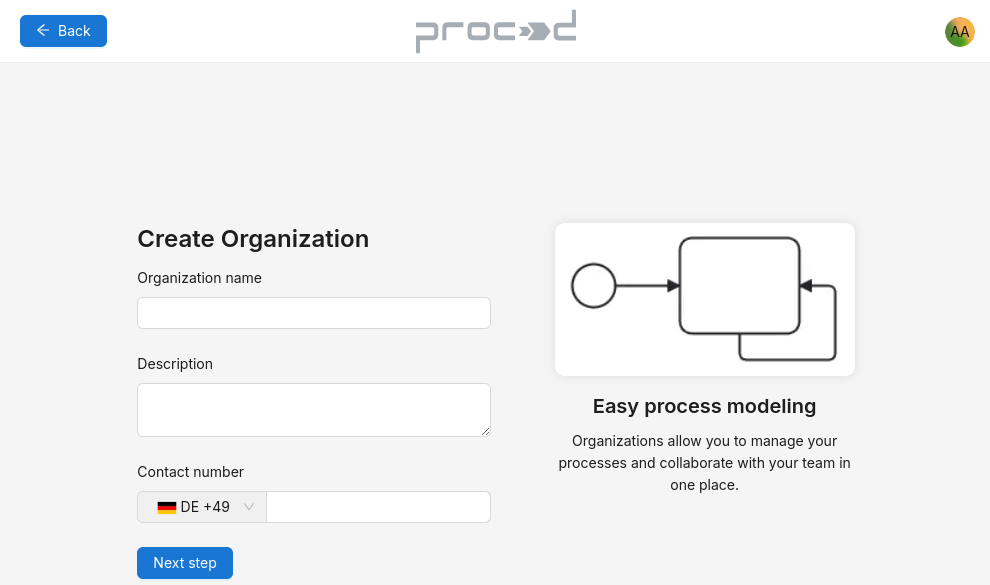
\includegraphics[scale=0.3]{images/create-organization-ui.png}
	\caption{Form for creating an organization environment.}
	\vspace{-1em} % Negative value to remove space
	\label{fig:prompt-fill-personal-information}
\end{figure}

\subsection{Adding Users to an Environment}

Adding users to an environment is simply done by creating a membership entry, with the
organization environment's \lstinline{id} and the user's \lstinline{id}.
However, the inviter typically doesn't know the invitee's internal \lstinline{id},
so they can use the invitee's email address instead.
The MS then sends an email to the invitee, with an invitation link that contains a token.
The link directs to a user to the MS, where the token is verified and the user is added to
the organization environment.
Additionally, if the inviter has the permissions for it, he can select roles for the new member.

% NOTE: mention that jwts have the drawback that they can't be revoked?'
The token in the invitation link is a JWT token, this way there is no need to store it.
The token contains the id's of the roles for
the invitees, the ID of the environment, and a reference to the invitee.
If the email the inviter provided is associated with a user, then the reference to the
invitee stores the user's \lstinline{id}, otherwise there is the risk, that the invitee
changes his email address, and the invitation link is no longer valid for him.
If the invitee's email address is not associated with a user, the token just stores his
email address.
In this case, when the invitee clicks on the link, he is first directed to the sign-in
page, and after he signs in he is redirected back to the invitation link.

% TODOFIG: show different options for inviting users

\subsection{Environment Selection}

% NOTE: maybe add footnote for url path

The selected environment is encoded in the URL's path like this:
\lstinline{https://staging.proceed-labs.org/<environment id>/...}.
Every view accessed by a user, where URL's path starts with an environment's id, will be
only related to that environment.
Each view can get this environment ID and fetch the appropriate assets.

\begin{lstlisting}[
  language=JavaScript,
  style=codestyle,
  caption={Example of a view processes based on the environment id.},
]
function ProcessesPage(props){
  const environmentId = props.params.environmentId; 

  const processes = getProcesses(environmentId);

  // render processes
}
\end{lstlisting}
% return (
%   <div>
%     {processes.map((process) => (
%       <ProcessCard process={process} />
%     ))}
%   </div>

Users can switch between environments by selecting them from a dropdown menu, that is
placed on the navigation bar.


\begin{figure}[H]
	\centering
	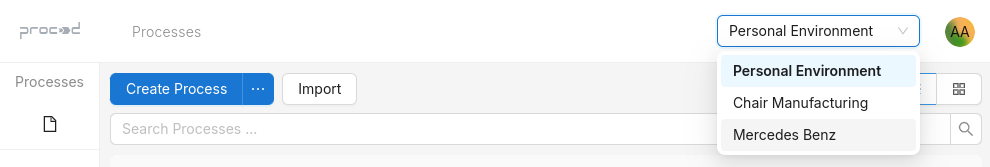
\includegraphics[scale=0.3]{images/select-environment.png}
	\caption{Selection of environments in the MS' navigation bar.}
	\vspace{-1em} % Negative value to remove space
\end{figure}

How everything was changed to support environmenst

- memberships
- verification (when envs are created by not signed in users)
- deletion - managing the env
- section for folders
- decide how to divide
- selection of envs
-

Environments are stored as an entry in the MS table

\subsection{Memberships}

\section{Roles}

% TODO: work on the intro 
Each role is now directly associated with an environment by storing an
\lstinline{environmentId} and its permissions only apply to in that environment.
Additionally, roles can now be associated to a folder, with the new field \lstinline{folderId}.


% TODO: decide where to put the role schema

\begin{lstlisting}[
  language=JavaScript,
  style=codestyle,
  caption={Example of a view processes based on the environment id.},
]
type Role = {
  environmentId: string;
  name: string;
  permissions: {
    Process?: number | undefined;
    Project?: number | undefined;
    Template?: number | undefined;
    Task?: number | undefined;
    Machine?: number | undefined;
    Execution?: number | undefined;
    Role?: number | undefined;
    User?: number | undefined;
    Setting?: number | undefined;
    EnvConfig?: number | undefined;
    RoleMapping?: number | undefined;
    Share?: number | undefined;
    Environment?: number | undefined;
    Folder?: number | undefined;
    MachineConfig?: number | undefined;
    All?: number | undefined;
  };
  description?: string | null | undefined;
  note?: string | null | undefined;
  expiration?: Date | null | undefined;
  }
\end{lstlisting}

\subsection{New Resources}

Folders and environments were added to the MS' resource list, and to the schema of
Roles, to allow for permissions to be set for them.
This way abilities can perform checks on these resources and enforce permissions like
% TODO: maybe instead of ref, write in the next chapter
described in \ref{cha:relatedwork:proceedroles}.

These resources, were also added to the MS' role management UI:

\begin{figure}[H]
	\centering
	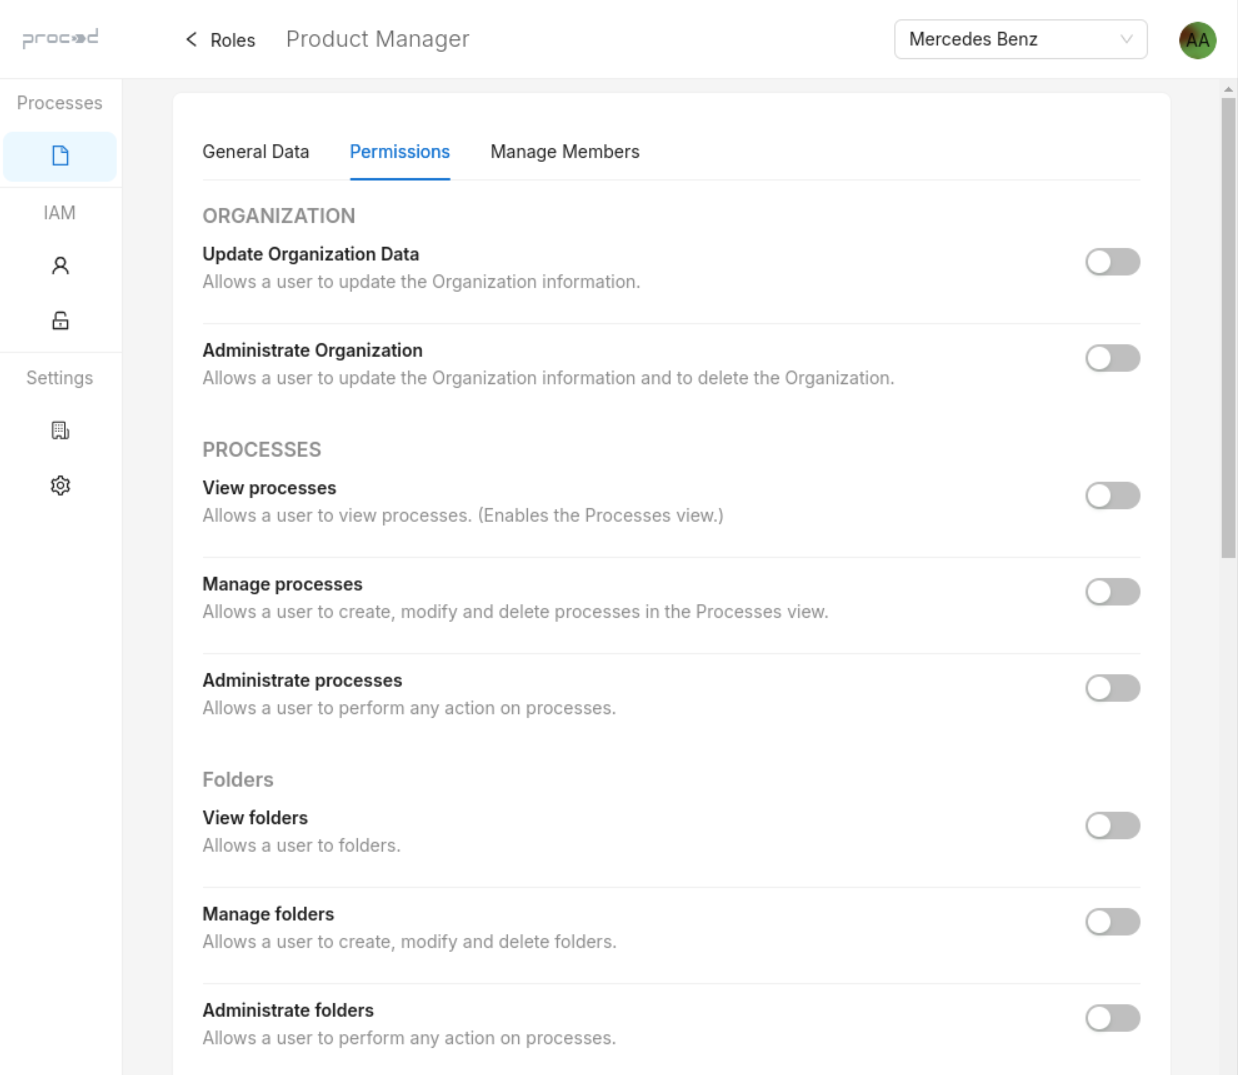
\includegraphics[scale=0.2]{images/role-permissions-view.png}
	\caption{Prompt to fill in personal information.}
	\vspace{-1em} % Negative value to remove space
	\label{fig:prompt-fill-personal-information}
\end{figure}



\subsection{Enforcing Roles in the MS}

Every action that a user can perform in an environment, is tied with a permission.
For this reason, every endpoint in the MS has to check permissions, fortunately, roles
were already implemented in the MS and every endpoint was already using abilities
\ref{cha:relatedwork:proceedroles:casl} to check permissions.
Abilities are built with the permissions stored in roles that a user has.
The only thing that was changed is that every endpoint receives the environment as an
argument, and uses the roles the user has in the environment for building his ability.

The function \lstinline{getCurrentEnvironment} was implemented in order to facilitate
getting a user's ability for an environment, it takes an environment ID and uses
functionality provided by NextAuth.js to know which user is calling the endpoint.

% NOTE: maybe remove the userError as if its not explained it might be confusing
\begin{lstlisting}[
  language=JavaScript,
  style=codestyle,
  caption={Example of an endpoint using an ability.},
]
async function(processValues, environmentId) {
  const { ability } = await getCurrentEnvironment(spaceId);

  if (!ability.can('create', toCaslResource('Process', newProcess))) {
    return userError('Not allowed to create this process');
  }

  ...
}
\end{lstlisting}

\subsection{Checking Permissions associated to a Folder}

The process of building abilities was modified to enable them to check a folder structure.
Abilities in the MS are built with a conditions matcher
\footnote{\url{https://casl.js.org/v6/en/advanced/customize-ability\#custom-conditions-matcher-implementation}},
which is a function that receives a conditions object and returns a function that checks
resource instances.
The conditions object is defined by each rule, which in turn are derived by the
permissions of roles as described in \ref{cha:relatedwork:proceedroles}.
If a rule allows an action on a resource instance and includes a conditions object, the
rule will only apply if the function returned by the conditions matcher evaluates to
\lstinline{true} when provided with the resource instance.

\begin{lstlisting}[
  language=JavaScript,
  style=codestyle,
  caption={Simple example of a conditions matcher in CASL.},
]
import { PureAbility, AbilityBuilder } from '@casl/ability';

function conditionsMatcher(conditions){
  if (conditions.hasToBeAdult){
    return (resourceInstance) => resource.age >= 18;
  }

  return (resourceInstance) => true;
}

function buildAbility(){
  const builder = new AbilityBuilder(PureAbility);

  builder.can('view', 'Process', { hasToBeAdult: true });

  return builder.build({ conditionsMatcher });
}

const ability = buildAbility();

ability.can('read', 'Post', { age: 17 }); // false
ability.can('read', 'Post', { age: 23 }); // true
\end{lstlisting}

% Since the conditions matcher only receives a conditions object, it can't take
% The conditions matcher was wrapped in a function that receives a representation of an
% environments folder structure.
% This function in turn returns a conditions matcher, which al

A simple representation of a folder structure is computed in the MS
and stored in a JSON serializable object.
Each key is a folder id, and its value is its parent's id.
Only the root folder's ID isn't contained in the object, as it has no parent.
This structure is used by the conditions matcher to check if a process or folder is a
descendant or ancestor of a folder.
These conditions can be set in the conditions object with the keys
\lstinline{$property_has_to_be_child_of} and \lstinline{$property_has_to_be_parent_of}.
% NOTE: turning is not the right word I think
These new conditions are used when turning role's permissions into rules.
The conditions matcher also includes a list of seen folders, in the case that the folder
structure is has an error and is circular.
\ref{lst:conditions-matcher-child-of} shows a simplified version of the implementation of
\lstinline{$property_has_to_be_child_of}, this implementation doesn't take into account
that the conditions object can have multiple conditions.

\begin{lstlisting}[
  language=JavaScript,
  style=codestyle,
  caption={Simplified implementation of \lstinline{$property_has_to_be_child_of} in the conditions matcher.},
  label={lst:conditions-matcher-child-of}
]

function conditionsMatcherFactory(folderStructure){
  function conditionsMatcher(conditions){
    if("$property_has_to_be_child_of" in conditions){
      return (resource: any) => {
        // Folder permissions are also applied to the folder itself
        if (
          (resource.__caslSubjectType__ as ResourceType) === 'Folder' &&
          resource.id === valueInCondition
        )
          return true;

        let currentFolder = resource.parentId;
        const seen = new Set<string>();
        while (currentFolder) {
          if (currentFolder === valueInCondition) return true;

          if (seen.has(currentFolder)) throw new Error('Circular reference in folder tree');
          seen.add(currentFolder);

          // Go up the folder structure
          currentFolder = folderStructure[currentFolder];
        }

        return false;
      };
    }
  }
}

function buildAbility(folderStructure, rootFolderId){
  const builder = new AbilityBuilder(PureAbility);

  builder.can('view', 'Process', {$property_has_to_be_child_of : rootFolderId });

  return builder.build({
    conditionsMatcher: conditionsMatcherFactory(folderStructure) 
  });
}
\end{lstlisting}

When a role is being used to build an ability, each permission for each asset is turned into a
rule.
When the role is associated to a folder, the rules for processes and folders, use
\lstinline{$property_has_to_be_child_of} in their conditions object, so that the
permissions cascade down the folder structure.
Additionally, if the role allows a user to view, either a folder or a process, a rule is
added, that allows the user to view all ancestors of the asset with
\lstinline{$property_has_to_be_child_of}.

